\problemname{Cars}

\illustration{0.3}{Self_driving_vehicle}{\href{https://commons.wikimedia.org/wiki/File:Self_driving_vehicle.jpg}{Picture} by Sammmerbatter via Wikimedia Commons, cc by-sa}%
\noindent
You work as an engineer at the leading self-driving car company Wayber. Wayber
just got approval from the government of Sweden for their cars to drive in the
streets of Stockholm. Unfortunately, all your tests so far have been with one
car at a time on a closed dirt track. You are not really prepared for what will
happen when two of the cars encounter each other in the city, and want to write
some code to handle this.

The cars are already good at staying inside the lines and turning. However,
they are not very good at detecting other moving vehicles. Fortunately, the
government of Sweden is so enthusiastic about self-driving cars that they have
banned all other forms of transportation in Stockholm, including human-driven
cars, biking, and walking. If you can just detect whether two cars will collide
you will be able to build a safe system.

You know that all cities consist of only north-south and east-west oriented
streets in a perfect grid, and all cars are perfect rectangular prisms. When
detecting collisions you only need to worry about cars traveling at a constant
speed without turning.

\begin{figure}[!h]
\centering
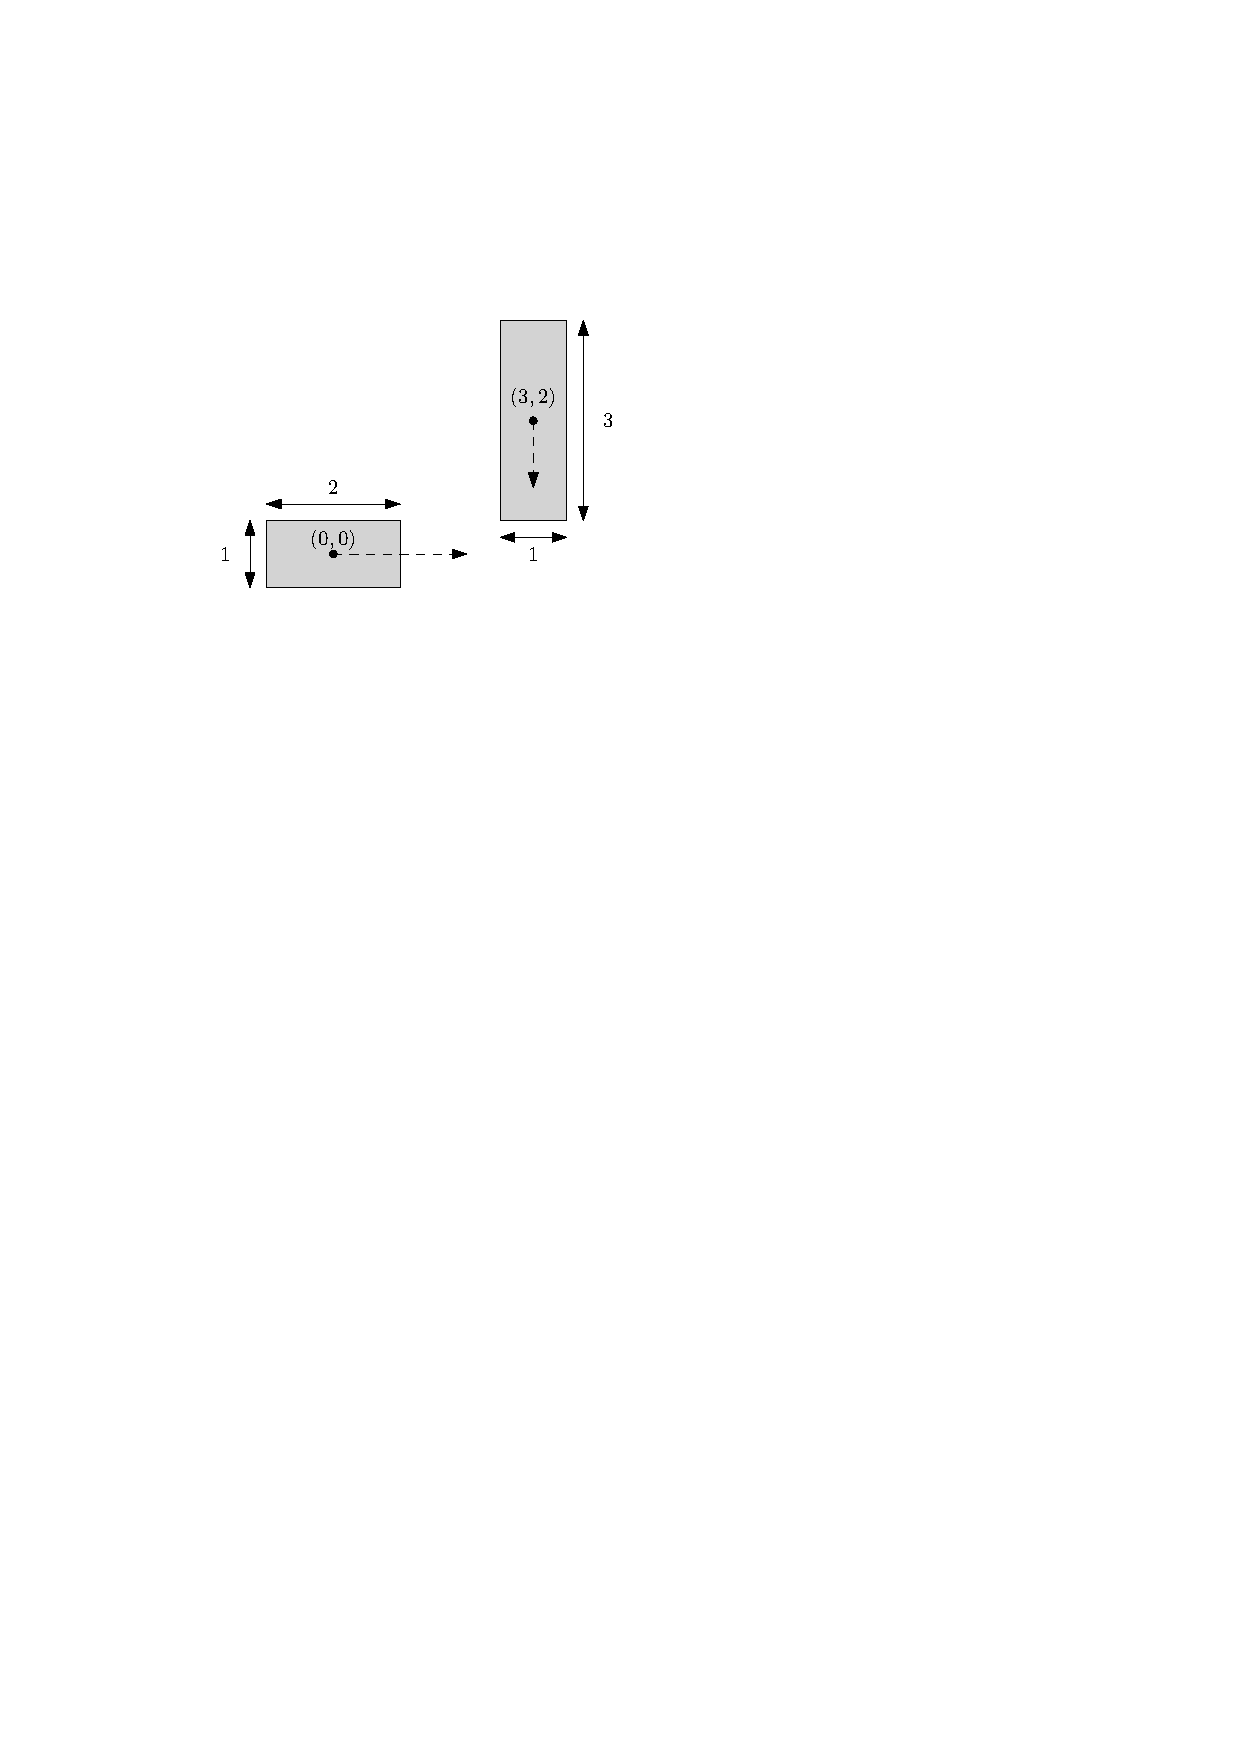
\includegraphics[width=0.35\textwidth]{sample1}
\caption{Illustration of Sample Input 1.}
\end{figure}

\section*{Input}

The first line of input contains an integer $1 \le t \le 10^4$, the
duration in seconds of the trajectory of the two cars.
Then follow the description of the trajectory of two cars.

A trajectory consists of a line containing a character $d$ and five
integers $x$, $y$, $s$, $w$ and $l$.
The starting position of the car is $(x,y)$ ($0 \le x, y \le 10^4$)
and its direction is $d$ which is either \texttt{N} (positive $y$
direction), \texttt{S} (negative $y$ direction), \texttt{W} (negative
$x$ direction) or \texttt{E} (positive $x$ direction).  The car is
travelling at a speed of $1 \le s \le 10^4$ units per second, is $1 \le
w \le 10^4$ units wide, and $1 \le l \le 10^4$ units long.

Cars start out centred on their starting coordinates and do not initially
overlap in a nonzero area.

\section*{Output}

For each line of input, output a line ``\texttt{crash}'' if the two cars will
crash or ``\texttt{safe}'' if they will not crash. If two cars overlap in an
area of size zero (only on an edge or corner) they do not crash.
